\providecommand{\isolatedBuild}[1]{#1}% fallback definition lets this file build normally
\isolatedBuild
{
\documentclass[11pt,letterpaper]{book}
\usepackage{import}

% This file must be found via the TEXINPUTS environment variable.
%\documentclass[11pt,letterpaper]{book}

% aleeper: I think these are needed for Paul's macros?
\usepackage{epsfig}
\usepackage{epstopdf}

%\makeatletter
%\typeout{The import path is \import@path}
%\makeatother

\usepackage{import}

\subimport{./}{packagesMitiguy.sty}
\subimport{./}{macrosMitiguy.tex}
\subimport{./}{PageStylesMitiguy.tex}
\subimport{./}{macrosLeeper.tex}


\pagestyle{plain}
\pagenumbering{arabic}

\begin{document}
\HandoutHeader{Robots Are Awesome}
%
%\vspace{-0.5pc}
\normalsize
\textColorBold{darkerBlue}{Statics of a Welding Robot}
\\[0.45pc]
}
%%%%%%%%%%%%%%%%%%%%%%%%%%%%%%%%%%%%%%%%%%%%%%%%%%%%%%%%%%%
%
Consider the 3-\textit{degree-of-freedom} (3-DOF) welding robot
consisting of a grounded link, \basis{N}, and rigid links \basis{A}, \basis{B}, and \basis{C}.
Revolute torque motors connect the links at points $A_o$, $B_o$, and $C_o$.
\\[0.45pc]
Right-handed, unitary, orthogonal vectors \uvecxyz{a} are fixed on body \basis{A}.
Right-handed, unitary, orthogonal vectors \uvecxyz{b} are fixed on body \basis{B} such that they are \textit{initially equal to} \uvecBasisxyz{a} and then subjected to a $+\uvecz{b}$ rotation of $\theta_B$.
Right-handed, unitary, orthogonal vectors \uvecxyz{b} are fixed on body \basis{C} such that they are \textit{initially equal to} \uvecBasisxyz{b} and then subjected to a $-\uvecz{c}$ rotation of $\theta_C$.
%
\\[0.45pc]
\begin{minipage}[t]{0.5\linewidth}
%
%
A load force $\bvec{F}_L = F_y \uvecy{c} + F_z \uvecz{c}$ is applied at point $C_1$.
\\[0.0pc]
Assume the links are uniform-density rods and relatively light (massless) compared to the applied loads.
\\[0.45pc]
{
\small
\begin{tabular}{|l|c|c|}
\hline Quantity                                                   & Symbol     & Value      % & (Initial) Value(s)
\\[0.0pc]\hline angle from \uvecx{a} to \uvecx{b} about $+\uvecz{b}$ & $\theta_B$ & $\degrees{60}$
\\[0.0pc]       angle from \uvecx{b} to \uvecx{c} about $-\uvecz{c}$ & $\theta_C$ & $\degrees{30}$
\\[0.0pc]\hline \uvecy{a} measure of distance from $A_o$ to $B_o$ & $L_A$     & \valueUnits{0.3}{m}
\\[0.0pc]       \uvecx{b} measure of distance from $B_o$ to $C_o$ & $L_B$     & \valueUnits{1.0}{m}
\\[0.0pc]       \uvecx{c} measure of distance from $C_o$ to $C_1$ & $L_C$     & \valueUnits{0.8}{m}
\\[0.0pc]\hline \uvecy{c} measure of load force at $C_1$ & $F_y$     & \valueUnits{800}{N}
\\[0.0pc]       \uvecz{c} measure of load force at $C_1$ & $F_z$     & \valueUnits{500}{N}
\\[0.0pc]\hline
\end{tabular}
}
\\[0.0pc]
An engineer might want to determine the motor torques and internal stresses in the links when the robot is in static equilibrium. As a first step, in this problem you will calculate some moments.
%
\end{minipage}
%
\hfill
%
\begin{minipage}[t]{0.45\linewidth}
\flushright
\vspace*{-0pc}
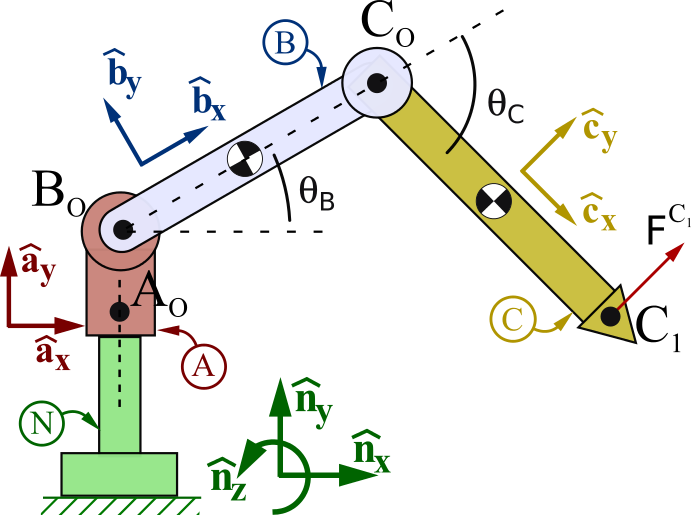
\includegraphics[width=0.99\linewidth]{robot_moment.png}
\end{minipage}
%
\\[0.45pc]
\begin{minipage}{0.33\linewidth}
{
% aleeper: I like asking for this one, since they don't actually need it in the
%          later calculations so it won't affect grading.
%          Also, they can't just copy b_R_c because the rotation sense is opposite.
\rotationTableEmpty{a}{b}{\hspace{1.3cm}}
%\simpleRotationZ{a}{b}{\theta_B}
}
\end{minipage}
\begin{minipage}{0.29\linewidth}
{
%\rotationTableEmpty{b}{c}{\hspace{1.3cm}}
\simpleRotationNegativeZ{b}{c}{\theta_C}
}
\end{minipage}
\begin{minipage}{0.33\linewidth}
{
\rotationTable{a}{c}
{~\cos(\theta_B - \theta_C)}{-\sin(\theta_B - \theta_C)}{0}
{~\sin(\theta_B - \theta_C)}{~~\cos(\theta_B - \theta_C)}{0}
{0}{0}{1}
}
\end{minipage}
%
\\[0.0pc]
\begin{enumerate}
\item Complete the rotation tables above.
\\[0.0pc]
%
\item Calculate \moment{\force{C_1}/C_o}, the moment of $\bvec{F}_L$ about $C_o$.
Express in terms of \uvecBasisxyz{c} and symbols in the table.
% aleeper: Doing the rotation table + this first question took me under 2 minutes;
%          this cross product is quite short.
\\[15.0pc]
\clearpage
\item Calculate \moment{\force{C_1}/B_o}, the moment of $\bvec{F}_L$ about $B_o$.
Express in terms of \uvecBasisxyz{c} and symbols in the table.
% aleeper: This second cross product took me 4-5 minutes. I decided to give them \dircos{b}{c}
%          so it doesn't affect their work on this part.
\\[30.0pc]
%
\item Express \posvec{A_o}{C_1} in terms of \uvecBasisxyz{a}.
%(That is, find the \uvecBasisxyz{a} measures of \posvec{A_o}{C_1}.)
The \uvecx{a} measure of \posvec{A_o}{C_1} is given to save you time.
\\[22.0pc]
%\textbf{Result: }
$\posvec{A_o}{C_1} = [L_B \cos(\theta_B) + L_C \cos(\theta_B - \theta_C) ]~\uvecx{a}
                   \plus[\;] \rule{7cm}{0.1mm} ~\uvecy{a}
                   \plus[\;] \rule{1.5cm}{0.1mm} ~\uvecz{a}$
%
\end{enumerate}
%
%
\isolatedBuild {
\rule{7in}{0.1mm}
\vfill
\end{document} }
